\chapter{Análise Bibliográfica sobre a Digitalização no Meio Educacional por Marcus Abrantes \label{chap:bibliometria:MarcusABR}}

\section{Planejamento do estudo}

A digitalização crescente tem transformado o comércio de informações. Quando bem empregada, possui o potencial de corrigir desigualdades, aperfeiçoar métodos e quebrar barreiras físicas. Este trabalho tem como objetivo analisar as últimas pesquisas e conclusões acerca de novas perspectivas que a digitalização trouxe ao meio educacional, bem como novas técnicas de ensino, dando atenção especial a gameficação. Uma técnica que surge inspirada em jogos para capturar a atenção dos estudantes e manter seu engajamento.

As seguintes perguntas foram usadas para nortear a pesquisa:
 
\begin{itemize}
    \item Qual a relevância e a atenção dada a pesquisa do uso de tecnologia na educação nos últimos anos?
    \item A gameficação tem sido considerada como uma técnica pertinente na avaliação de métodos de ensino?
    \item Nos últimos anos com o evento da pandemia, este assunto tem alçado maior importância, dados os desafios apresentados?
\end{itemize}

\subsection{Limitações} O trabalho foi desenvolvido ao decorrer de uma semana, empregando por volta de 5 a 10 horas.

\section{Coleta de dados}

A coleta de dados feita usando o mecanismo Web of Science no dia 09 de fevereiro de 2022, acessado por meio do Portal de Periódicos da CAPES.

\subsection{Query de Busca}

Para a busca dos artigo, foi usada a seguinte query:
\begin{verbatim}
educ*
and
(digital*  or gamific*)
and
improv*
and
learn*
\end{verbatim}

\subsubsection{Explicação para os termos de busca usados}

Tendo como tópico central a educação o termo \texttt{educ*}  foi utilizado. Dado o enfoque no meio digital, usa-se o termo \texttt{digita*}, para aumentar a abragência de forma a incluir a gameficação, o termo \texttt{or} \texttt{gamefic*}. Como este trabalho tem enfoque nas melhorias trazidas pelo meio digital, e não nas consequências e desafios de seu uso, é adcionado o termo \texttt{improv*}. Por fim, para reduzir a generalidade e tratar mais do contexto de aprendizado, também foi o usado o termo \texttt{learn*}


\subsection{Registros recuperados}

 Os 7795 registros obtidos na busca podem ser encontrados no \href{https://github.com/jhcf/Comput-Experim-20212/blob/main/experiments/MarcusABR/PesquisaBibliometrica/savedrecs.txt}[link]
Foi utilizado o recurso \textit{Exportar registros para arquivo de texto sem formatação}, com todos as 29 opções de campo disponíveis. Os 7795 registros foram recuperados em grupos de 1000 para posteriormente serem concatenados e analisados em conjunto.

\section{Análise dos dados}

\subsection{Filtragem de registros}


O registo inicial do \dataset\ possui 7795 documentos. Para reduzir seu número e efetuar a a análise apenas sobre aqueles mais pertinentes, foram aplicados filtros. Primeiramente, foram excluídos todos os registros não caracterizados como artigos publicados em revistas científicas. Após isso, usando a lei de Bradford, os documentos foram reduzidos para apenas as fontes principais. Após a filtragem 1124 arquivos foram selecionados.

\subsection{Análise descritiva do \dataset\   }

Constam as informações gerais sobre os conjuntos de dados:
\begin{description}
    \item [\textit{Timespan}] Os documentos obtidos na busca após a filtragem foram publicados entre o período de 1991 até 2022.
    \item [\textit{Sources (Journals, Books, etc)}] Os artigos possuem ao todo 29 fontes diferentes, sendo assim, em média, 39 artigos por revista.
    \item [\textit{Average years from publication}] A média de tempo de publicação dos artigos é de 4,26 anos.
    \item [\textit{Average citations per documents}] A média de citações por documentos é 18,35.
    \item [\textit{Average citations per year per doc}] Após o ano de sua publicação, cada um dos dos artigos foi citado em média 2713 vezes por ano.
    \item [\textit{References}] Ao todo, foram feitas 46553  referências por entre os artigos coletados.
    \item [\textit{Keywords Plus (ID)}] 1828 palavras chaves do tipo ID (Keyword Plus).
    \item [\textit{Author's Keywords (DE)}]  3211 palavras chaves escolhidas pelos autores dos artigos.

    \item [\textit{Authors}]  Ao todo, foram encontrados 3874 autores no dataset.
    \item [\textit{Author Appearances}] Os 3874 nomes apareceram 4543 vezes nos documentos.
    \item [\textit{Authors of single-authored documents}] Dos 3874 autores, 81 escreveram artigos individualmente.
    \item [\textit{Authors of multi-authored documents}] Dos 3874 autores, 3793 são autores de artigos escritos em colaboração com outros.
    \item [\textit{Single-authored documents}] Dos 1124 documentos, 85 foram escritos individualmente, os 1039 restantes foram produzidos em co-autoria.
    \item [\textit{Documents per Author}] A média de documentos por autor é de 0.29.
    \item [\textit{Authors per Document}] A média de autores por documento é de 3.45.
    \item [\textit{Co-Authors per Documents}] As 4543 aparições de autores se distribuem em 4.04 por documento.
    \item [\textit{Collaboration Index}] O indíce de colaboração (total de autores em artigos escritos em co-autoria / total de artigos escritos em co-autoria) é de 3,65.
\end{description}

\subsection{Evolução da Produção Científica}



\begin{figure}[ht]
    \centering
    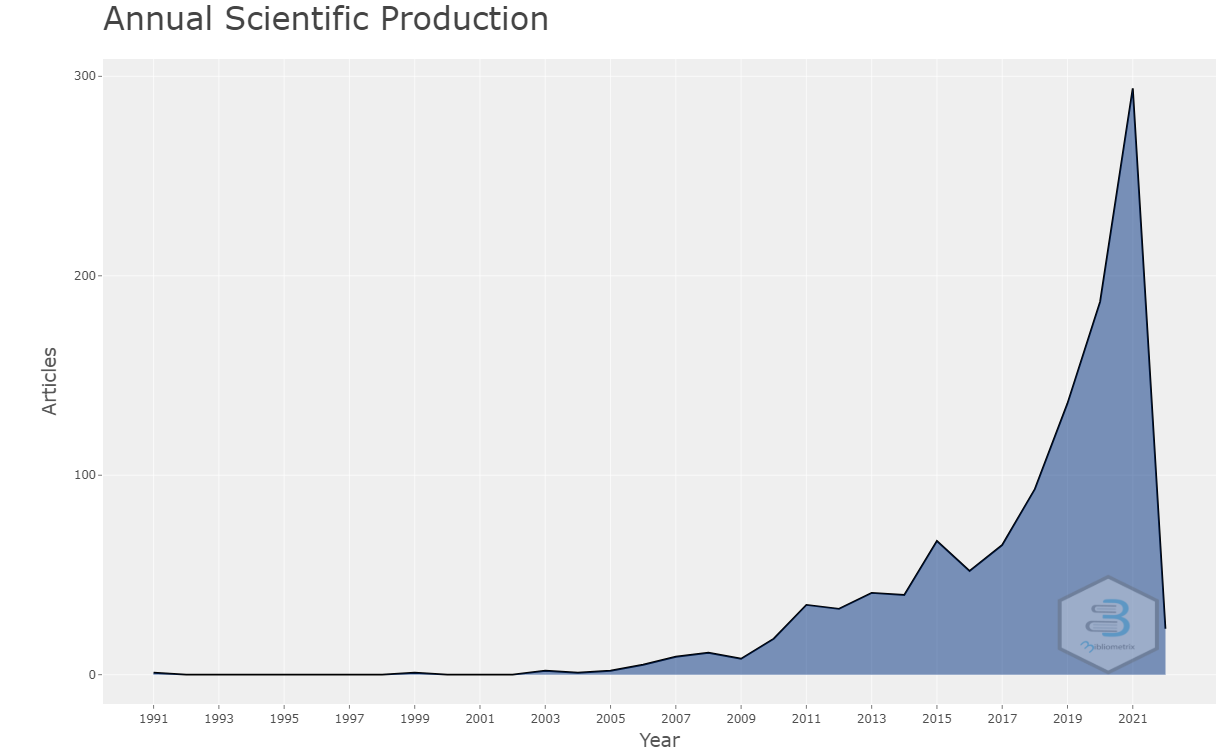
\includegraphics[width=12cm]{experiments/MarcusABR/PesquisaBibliometrica/Imagens/newplot.png}
    \caption{Evolução da produção científica no \dataset\ }
    \label{fig:eddi-evolucao}
\end{figure}

Conforme demonstra o gráfico \ref{fig:eddi-evolucao} houve uma crescente a partir de 2017, alcançando o seu age durante os anos da pandemia entre 2019-2021. Durante esses anos, o ensino a distância foi empregado de forma massiva ao redor do mundo, o que evidenciou não só as dificuldades da educação em meios digitais, mas também as muitas vantagens que ainda não eram exploradas na tecnologia para aprimorar o estudo.
Por conseguinte, as pesquisas cresceram rapidamente, abrindo espaço para questões sobre como deve ser o ensino nos próximos anos. A utilização de técnicas como a gameficação e a exploração de métodos que substituam as clássicas técnicas de ensino tendem a apenas crescer com o passar dos anos.


\subsection{Evolução das Citações}


A figura em \ref{fig:eddi-citation-year} mostra o número médio de citações feita por anos. A maior amplitude se encontra entre os anos de 2011 até o ano de 2017, demonstrando que houve um aumento no comércio científico de informações e na troca de referências. No ano de 2010 foi quando o gráfico encontrou seu pico, evidenciando que artigos de renome surgiram nesse ano.

\begin{figure}[ht]
    \centering
    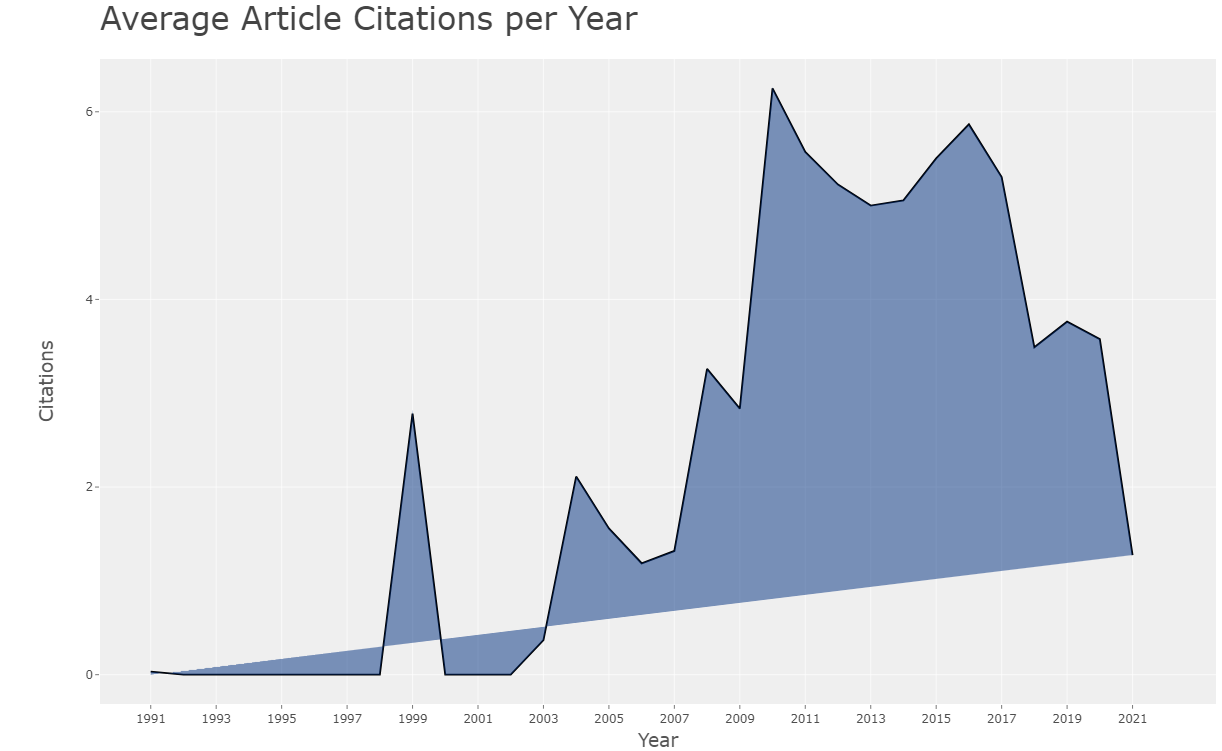
\includegraphics[width=12cm]{experiments/MarcusABR/PesquisaBibliometrica/Imagens/newplot(1).png}
    \caption{Evolução das citações por ano no \dataset\ }
    \label{fig:eddi-citation-year}
\end{figure}

\subsection{\textit{Gráfico de três campos}}

Na figura está um gráfico de três campo que relaciona as fontes de com autores e palavras chaves.

\begin{figure}[ht]
    \centering
    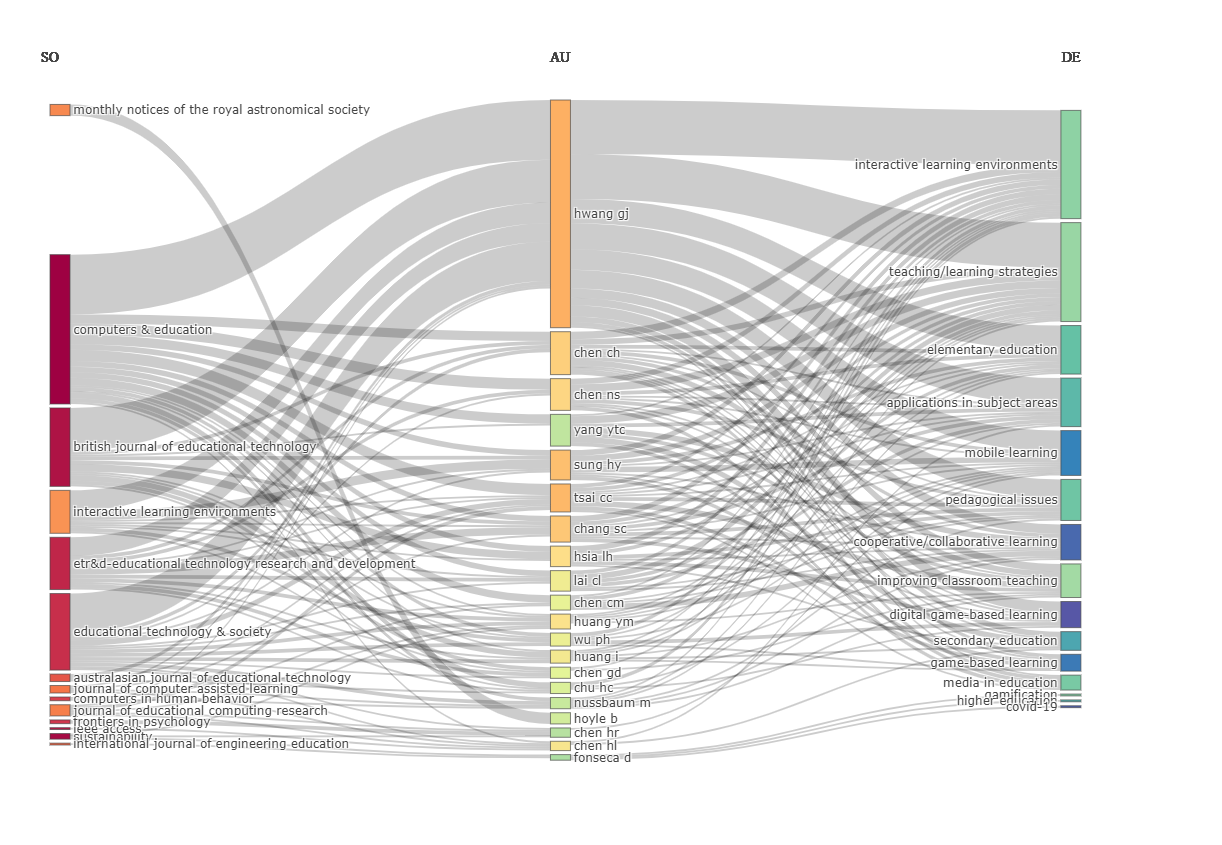
\includegraphics[width=12cm]{experiments/MarcusABR/PesquisaBibliometrica/Imagens/newplot(3).png}
    \caption{Gráfico de três campos analisando fonte, autor e palavras chave}
    \label{fig:eddi-three-field}
\end{figure}

Observando o gráfico \ref{fig:eddi-three-field} é possível perceber que a maior fonte de conhecimento acerca do assunto advém da revista computers \& education, sendo a que mais se relaciona com autores. Em especial, o autor \textit{hwang dj} demonstra ter trabalho em diversas revistas no campo de educação digital.

No campo das palavras chaves em \ref{fig:eddi-three-field}, se evidencia como o maior é interesse é por ambiente de aprendizado interativo, assim como estratégia de ensino e aprendizado. Isto demonstra que muitas pesquisas estão surgindo acerca de novos métodos de ensino e novas formas de lidar com a educação digitalmente. Ainda é possível perceber a relevância do termo \textit{elementary education}, indicando que possivelmente essas novas estratégias se desenvolvem no ensino fundamental.

Por fim, alguns termos se relacionam com aprendizado inspirado em jogos digitais, demonstrando que a pesquisa sobre gameficação tem encontrado relevância nas revistas científicas.



